\documentclass[10pt,compress]{beamer}
\usepackage{amsmath}
\usepackage{cmbright}
\usepackage{url}
\usepackage{ucs}
\usepackage[utf8x]{inputenc}
\usepackage[ngerman]{babel}
\usepackage{bbm}
\usepackage{ulem}
\usepackage{multicol}
\usepackage{comment}
\usepackage{setspace}
\usepackage{color}
\usepackage{hyperref}
\usepackage{bookman}
\usepackage{wasysym}

\usetheme{Boadilla}
\setbeamertemplate{footline}%{infolines theme}

\usecolortheme{lily}
\usefonttheme{serif}
\useinnertheme{circles}
\setbeamercovered{transparent}
\beamertemplatenavigationsymbolsempty

\definecolor{darkgreen}{rgb}{0,0.5,0}

\hypersetup{
    bookmarks=true,
    unicode=true,
    pdftoolbar=true,
    pdfmenubar=true,
    pdffitwindow=false,
    pdfstartview={FitH},
    pdftitle={Ethanol -- Aufnahme und Abbau},
    pdfauthor={Michael Hartmann},
    pdfsubject={Vortrag über den zeitlichen Verlauf der Blutalkoholkonzentration im Blut},
    pdfcreator={vim},
    pdfproducer={pdflatex},
    pdfkeywords={Blutalkoholkonzentration} {Ethanol} {Aufbau} {Abbau},
    pdfnewwindow=true,
    colorlinks=true,
    linkcolor=black,
    citecolor=green,
    filecolor=magenta,
    urlcolor=darkgreen
}



\title{UNIX Dateirechte}
\institute{Linux User Group Augsburg}
\author{Michael Hartmann}
\date{7. Oktober 2015}


\begin{document}

\begin{frame}
    \titlepage
\end{frame}


\frame {
    \frametitle{Sicherheitskonzept}

    \only<1>
    {
        \begin{center}
        \Huge Wie funktioniert eigentlich {\it Sicherheit} auf Computern?
        \end{center}
    }
    \only<2>
    {
        \begin{center}
        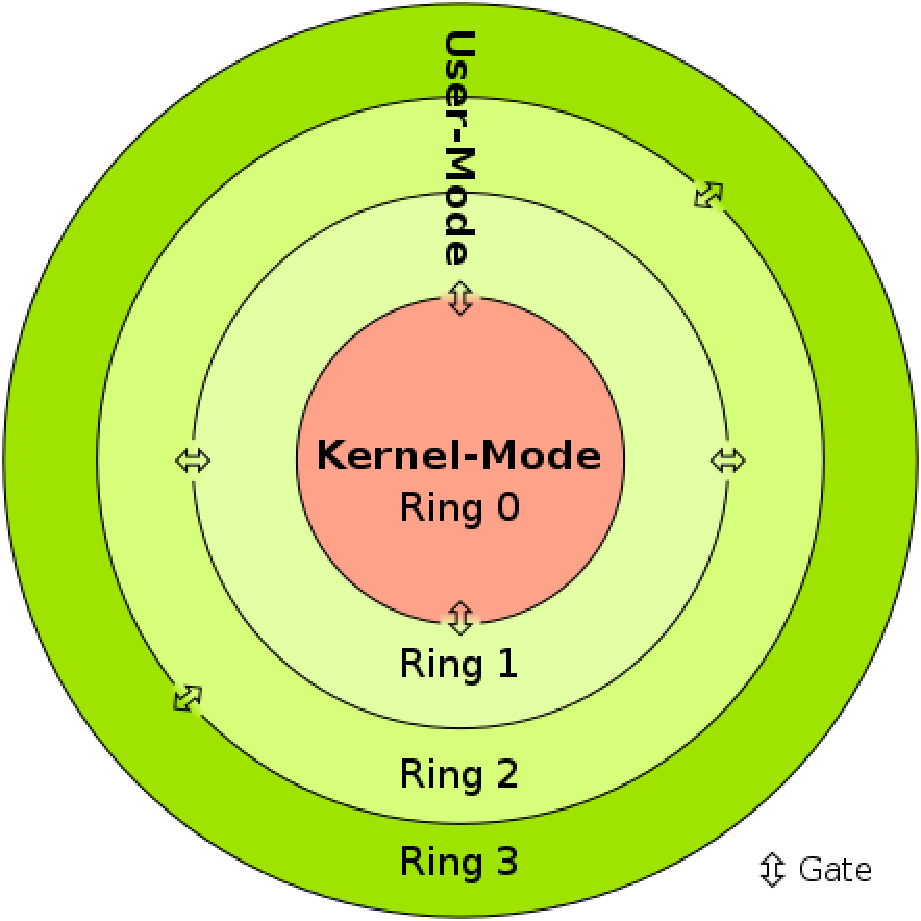
\includegraphics[scale=0.4]{ring.pdf}
        \end{center}

        \vfill
        \vfill
        \noindent\rule{10cm}{0.4pt}
        \url{https://de.wikipedia.org/wiki/Ring_\%28CPU\%29}
    }
}

\frame {
    \frametitle{CPU-Ringe}
    
    Funktionsweise:
    \begin{itemize}
    \item Ring (Domain): Sicherheitsstufe auf der CPU
    \item innerer Ring: darf alles
    \item äußere Ringe: eingeschränkter Befehlssatz
    \item Linux benutzt nur zwei Ringe (Kernel- und Benutzer-Modus)
    \end{itemize}
    
    \vfill
    \pause
    Vorteile:
    \begin{itemize}
    \item Ringe ermöglichen Betriebssystem Sicherheitsmechanismen
    \item Einschränken von Hardware-Zugriff
    \item Abschotten von unterschiedlichen Prozessen
    \item ermöglicht Virtualisierung (in der Theorie...)
    \end{itemize}
}


\frame {
    \frametitle{Systemaufrufe}

    \begin{center}
    \only<1>
    {
        \Huge Wie greift dann ein Prozess auf Hardware zu?
    }
    \only<2>
    {
        \Huge Systemaufrufe!
    }
    \end{center}
}


\frame {
    \frametitle{Systemaufrufe}

    Ablauf:
    \begin{enumerate}
    \item Prozess legt an einer bestimmten Stelle Zahlenwert / Daten ab
    \item Prozess löst Software-Interrupt ab
    \item Prozess wird unterbrochen, CPU wechselt in Ring 0
    \item Funktion im Kernel erledigt Aufgabe
    \item CPU wechselt wieder in Ring 3, Prozess wird weiter ausgeführt
    \end{enumerate}

    \vfill
    \pause
    Vorteile:
    \begin{itemize}
    \item Prozess hat zu keinem Zeitpunkt Zugriff auf Hardware
    \item Kernel kann entscheiden, ob Prozess Zugriff auf {\it Ressource} bekommt
    \end{itemize}
}

\frame {
    \frametitle{Systemaufrufe}

    \only<1>
    {
        \begin{center}
        \Huge Was sind denn solche Systemaufrufe?
        \end{center}
    }
    \only<2>
    {
        Auswahl von Linux-Systemaufrufen:
        \begin{itemize}
        \item \texttt{open}
        \item \texttt{read}
        \item \texttt{write}
        \item \texttt{close}
        \vfill
        \item \texttt{kill}
        \item \texttt{chdir}
        \item \texttt{chmod}
        \vfill
        \item \texttt{sendmsg}
        \item \texttt{recvmsg}
        \end{itemize}
    }
}

\frame {
    \frametitle{UNIX Dateirechte}

    \begin{center}
    {\Huge Wer darf was?}
    \end{center}

    \pause
    Wer:
    \begin{itemize}
    \item \textbf{u}ser (Eigentümer)
    \item \textbf{g}roup (Gruppe)
    \item \textbf{o}ther (alle anderen)
    \end{itemize}

    \vfill
    \pause
    Was:
    \begin{itemize}
    \item \textbf{r}ead (lesen)
    \item \textbf{w}rite (schreiben)
    \item e\textbf{x}ecute (ausführen)
    \item setuid, setgid, sticky bit
    \end{itemize}
}

\frame {
    \frametitle{chmod}

    Oktal: \quad
    \begin{tabular}{c|c}
    Berechtigung & Zahl \\
    \hline 
    lesen     & 4 \\
    schreiben & 2 \\
    ausführen & 1
    \end{tabular}

    \vfill
    Ändern von Dateirechten:
    \begin{itemize}
    \item \texttt{chmod u=rw  datei}
    \item \texttt{chmod u+rwx datei}
    \item \texttt{chmod g-rx  datei}
    \item \texttt{chmod o+r   datei}
    \item \texttt{chmod a+r   datei}
    \item \texttt{chmod 700   datei}
    \end{itemize}
}

\frame {
    \frametitle{Grundlegende Rechte}

    Lesen:
    \begin{itemize}
    \item Dateien: Benutzer darf Datei lesen
    \item Verzeichnisse: Benutzer darf Inhalt eines Verzeichnisses auslesen
    \end{itemize}

    \vfill
    \pause
    Schreiben:
    \begin{itemize}
    \item Dateien: Benutzer darf Datei schreiben
    \item Verzeichnisse: Benutzer darf Dateien erstellen, umbennen, löschen und deren Dateireche ändern
    \end{itemize}

    \vfill
    \pause
    Ausführen:
    \begin{itemize}
    \item Dateien: Benutzer darf Programm ausführen
    \item Verzeichnisse: Benutzer darf in das Verzeichnis wechseln
    \end{itemize}
}

\frame {
    \frametitle{setuid/setgid}

    setuid (\texttt{s}):
    \begin{itemize}
    \item Dateien: ausführbares Programm wird mit Rechten des Besitzers der Datei ausgeführt
    \item Verzeichnisse: ignoriert (Linux)
    \end{itemize}

    \vfill
    \pause

    setgid (\texttt{s}):
    \begin{itemize}
    \item Dateien: ausführbares Programm wird mit Rechten der Gruppe der Datei ausgeführt
    \item Verzeichnisse: neu erstellte Dateien erben die Gruppen-ID
    \end{itemize}

    \vfill
    \pause

    sticky bit (\texttt{t}):
    \begin{itemize}
    \item Dateien: ausführbares Programm bleibt nach Beenden im Arbeitsspeicher (historisch)
    \item Verzeichnisse: nur noch der Besitzer einer Datei darf diese löschen (Beispiel: \texttt{/tmp})
    \end{itemize}
}

\frame {
    \frametitle{Hackles}

    \begin{center}
    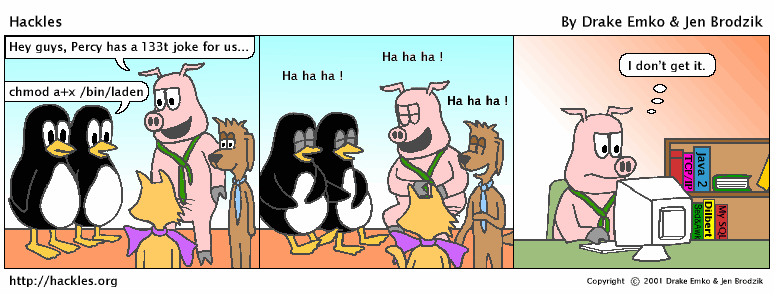
\includegraphics[scale=0.4]{hackles.png}
    \end{center}

    \vfill
    \vfill
    \noindent\rule{10cm}{0.4pt}
    \url{http://hackles.org/cgi-bin/archives.pl?request=65}
}

\frame {
    \begin{center}
    \Huge Vielen Dank für die Aufmerksamkeit :)
    \end{center}
}

\end{document}
